\documentclass[a4paper,11pt]{article}
\usepackage[utf8]{inputenc} % Required for inputting international characters
\usepackage[T1]{fontenc} % Output font encoding for international characters
\usepackage[italian]{babel} % Italian dictionary
\usepackage{siunitx} % SI
\usepackage{amsmath}

\usepackage{graphicx} % cooler tables
\usepackage{wrapfig} % tables/images alignment

\usepackage{bm}
\usepackage{tikz}
\usepackage{hhline}
\usepackage{listings}

\usepackage[margin=2cm, includefoot]{geometry} % Modify margins
\usepackage{fancyhdr}
\usepackage{rotating}
\usepackage[hidelinks]{hyperref} % Hyperlinks

\usepackage[none]{hyphenat}% Non spezza le parole nelle tabelle
\usepackage{array}

\usepackage{graphicx} % Required for figures
\usepackage{float}
\usepackage{caption}
\usepackage{subcaption}

%pagestyle
\pagestyle{fancy}
\fancyhead{}
\fancyfoot{}
\fancyfoot[R]{\thepage}
\renewcommand{\headrulewidth}{0pt}


\usepackage{xfrac}
\usepackage{amssymb}

\usepackage{multicol}
\usepackage{multirow}

\usepackage[toc, page]{appendix}
\usepackage{booktabs}

% THIS IS DUMB BUT I'M IN A HURRY
\newcommand\V{ \,\si{\volt}}
\newcommand\kOhm{ \,\si{k}\Omega}
\newcommand\MOhm{ \,\si{M}\Omega}
\newcommand\kHz{ \,\si{k\Hz}}
\newcommand\Hz{ \,\si{\Hz}}
\newcommand\nF{\,\si{n\farad}}
\newcommand\us{\,\si{u\s}}
\newcommand\sh{\text{sh}}
\newcommand\out{\text{out}}
\newcommand\inp{\text{in}}


\usepackage{circuitikz}

\begin{document}

%-------------------------------------------------------------------------------------------------------------------------------------------
%	TITLE PAGE
%-------------------------------------------------------------------------------------------------------------------------------------------
\begin{titlepage}
	\newcommand{\HRule}{\rule{\linewidth}{0.5mm}}
	\center
	% ------------------------------------------------
	%	Headings
	%------------------------------------------------

	\textsc{\LARGE Univeristà Degli Studi Di Padova}\\[1.5cm]
	\Large Corso Di Laurea In Fisica\\[0.5cm]

	\textsc{\large Laboratorio Di Fisica}\\
    A.S. 2020/2021 --- Canale A-L \\[0.5cm]

	%------------------------------------------------
	%	Title
	%------------------------------------------------

	\HRule\\[0.4cm]

	{\huge\bfseries Catena Elettronica}\\[0.4cm]

	\HRule\\[1.5cm]

	%------------------------------------------------
	%	Author(s)
	%------------------------------------------------

	\begin{minipage}{0.4\textwidth}
		\begin{flushleft}
			\large
			\textsc{Cigagna Simone}\\
			\textsc{1193992}
			simone.cigagna@studenti.unipd.it
		\end{flushleft}
	\end{minipage}
	~
	\begin{minipage}{0.4\textwidth}
		\begin{flushright}
			\large
			\textit{Docenti}\\
			Prof. A. Garfagnini\\
			Prof. M. Lunardon
		\end{flushright}
	\end{minipage}

	%------------------------------------------------
	%	Date
	%------------------------------------------------

	\vfill\vfill\vfill % Position the date 3/4 down the remaining page

	{\large \textsc{Data esperienza}\\
  13/01/2021 - 14/01/2021}

\end{titlepage}

\cleardoublepage


	%------------------------------------------------
	%	Obiettivi
	%------------------------------------------------
\section{Obiettivi}
In questa esperienza ci si propone di realizzare una versione semplificata di
una catena elettronica per un rilevatore di radiazione, costituita da un
preamplificatore, uno shaper e un amplificatore non invertente.
In particolare, si studia la linearità e le risposta in frequenza
dei componenti presi singolarmente, oltre che della catena completa.
\begin{figure}[h]
\centering
    \begin{circuitikz}[scale=0.7, transform shape, use fpu reciprocal]
      % preamp
      % BOX
      \draw[black, dashed] (-1,-3) rectangle (6,4.5)
        (0.5,-3) node[above]{Preamplificatore};
      \draw(0,2) node[above,font=\boldmath]{$V_{in}$};
      \draw(0,0) node[ground]{}
      (0,2) to[american voltage source,l=$V_{gen}$,font=\boldmath] (0,0) % Generator
      (0,2) to[R,l=$R_{1}$,font=\boldmath] (2,2) % R1
      to[R,l_=$R_f$,font=\boldmath] (5.5,2) % R_f
      to[short] (5.5,3.5)
      to[C,C=$C_f$,font=\boldmath] (2,3.5) % C_f
      to[short] (2,0);
      \draw(4,-0.5) node[op amp] (OA1){$OA_{1}$} % OPAMP1
      (OA1.-)-- (2,0)
      (OA1.+)-- (2,-1)
      (2,-1) to (2,-2) node[ground]{} % OPAMP1 ground
      (OA1.out)-- (5.5,-0.5)
      (5.5,-0.5)-- (5.5,2);
      % shaper
      % BOX
      \draw[black, dashed] (6.5,-3) rectangle (16.8,4.5)
        (8.2,-3) node[above]{Shaper $CR-RC$};
      \draw(5.5,1) to (7,1)
        (7,1) to[C,l_=$C_{sh1}$,font=\boldmath] (9,1)
          (7,1)-- (7,2.5) to[R,l_=$R_{pz}$,font=\boldmath] (9,2.5)-- (9,1)
          (9,1)-- (10,1) to[R,l_=$R_{sh1}$,font=\boldmath] (10,-1) to (10,-1) node[ground]{};
      \draw(12,1.5) node[op amp] (OA2){$OA_{2}$}
        (OA2.+)-- (9,1)
        (OA2.-)-- (10.5,2)-- (10.5,3.5)-- (13.5,3.5)-- (13.5,1.5)
        (OA2.out)-- (14,1.5) to[R,l=$R_{sh2}$,font=\boldmath] (15.5,1.5)-- (16,1.5)
          (16,1.5) to[C,l_=$C_{sh2}$,font=\boldmath] (16,-0.5) node[ground]{};
      % ampli
      % BOX
      \draw[black, dashed] (17.2,-3) rectangle (22.5,4.5)
        (18.5,-3) node[above]{Amplificatore};

      \draw(20,-0.5) node[op amp] (OA3){$OA_{3}$}
        (OA3.+)-- (17.5,-1)-- (17.5,1.5)-- (16,1.5)
        (OA3.-)-- (18.5,0)-- (18.5,1.5) to[R,l=$R_{a2}$,font=\boldmath] (21,1.5)-- (21,-0.5)
        (18.5,1.5) to[R,l=$R_{a1}$,font=\boldmath] (18.5,3)
        (18.5,3) node[ground, yscale=-1]{}
        (OA3.out) to[short,-*,l=$V_{out}$,font=\boldmath] (22,-0.5);

    \end{circuitikz}
    \caption{\footnotesize Schema a variabile concentrate della catena elettronica completa.}
\end{figure}\label{fig:circ_tot}

	%------------------------------------------------
	%	Apparato Sperimentale
	%------------------------------------------------

    % TODO: specifica sigma_k oscilloscopio

\section{Apparato Sperimentale}
Gli strumenti che si utilizzano nel corso dell'esperienza sono i seguenti:
\begin{itemize}
	\item Multimetro digitale Tenma 72-13430
  	\item Oscilloscopio Picoscope 2204A con due sonde di compensazione e con un generatore di funzioni incorporato
  \item Due circuiti integrati TL082 contenenti due amplificatori operazionali
        ciascuno
	\item Breadboard con scheda di alimenatazione $-12/0/12\, \si{\volt}$
	\item Resistori e condensatori di diversa taglia
\end{itemize}

\section{Preamplificatore Di Carica}
In questa sezione si verifica l'effetto di integrazione di carica del primo modulo della catena elettronica, ovvero un circuito $RC$ con un amplificatore operazionale invertente. Inoltre, si verifica la linearità della tensione massima in uscita ripetto alla carica che raggiunge il condensatore e si studia la risposta in frequenza del circuito.

\subsection{Configurazione Sperimentale}\label{sec:preamp_config_sperim}
Viene assemblato sulla breadbord il primo modulo in Figura~\ref{fig:circ_tot} utilizzando le
resistenze e la capacità riportati in Tabella~\ref{tab:preamp_misure} e si collegano due
sonde di compensazione 10X nei punti $V_{\text{in}}$ e $V_{\text{out}}$ in modo da
poter rilevare il segnale di tensione nei canali A e B dell'oscilloscopio. L'amplificatore viene alimentato con la scheda di alimentazione a $\pm 12\V$ e si aggiungono due capacità da $100\nF$ tra i pin dell'operazionale riservati all'alimentazione e la massa, in modo da attenuare eventuali fenomeni di oscillazione dovuti all'alto guadagno.  Si configura quindi il generatore di
%\begin{wrapfigure}{r}{0.4\textwidth}
 %\ \centering
  %\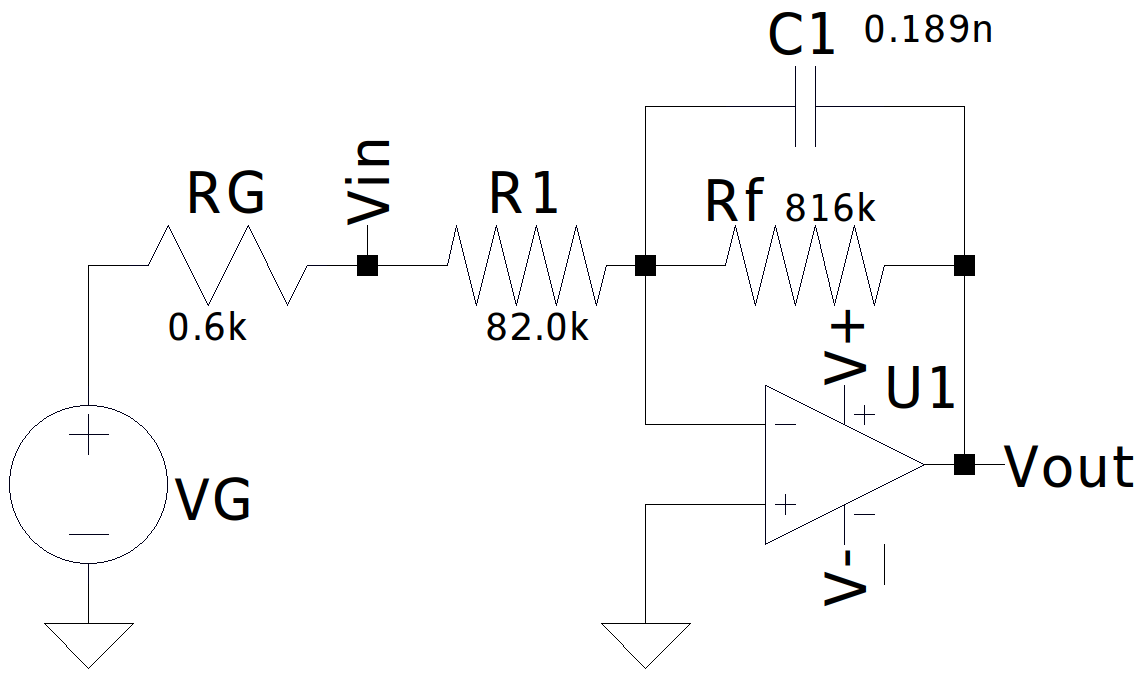
\includegraphics[width=0.38\textwidth]{../preamp/images/circuito}
  %\\caption{\footnotesize Schema a variabili concentrate del circuito preamplificatore.}
  %\\vspace{-10pt}
%\end{wrapfigure}\label{fig:preamp_circuito}%-----------------------------
funzioni incluso nel Picoscope in modo da
generare un impulso di tensione negativo di $-1\V$, partendo da un'quadra e
configurando il duty cycle al $99.5 \%$. In questo modo, selezionando una
frequenza di $1\kHz$, si ottiene una durata dell'impulso di $5\,\si{u\s}$ e,
tenendo conto della resistenza $R_{\text{in}}$ in serie, si può interpretare
come un impulso di corrente con una resistenza in parallelo, simulando quindi
l'output di un rilevatore di radiazione. Si nota però che, a causa dei limiti
tecnici del PicoScope 2204A, la durata del segnale non è stabile e non si presenta
come un'onda quadra perfetta, ma appare smussata.
Tutte le misure vengono quindi eseguite mettendo prima in pausa l'acquisizione
del segnale e si assume come valore del priodo quello nominale, con un'incertezza
sistematica  $\sigma_{T}=3\%$.%------------------------------
\renewcommand{\arraystretch}{1.1}
\begin{table}
\centering
\setlength{\tabcolsep}{10pt}
\begin{tabular}{ |c|c|c|  }
\hline
\multicolumn{3}{|c|}{Misure dirette dei componenti del circuito} \\
\hline
Label      & Valore & F.S.\\
\hline
$R_{1}$ & $82.0 \pm 0.4\,\si{k\Omega}$ &$200\,\si{k\Omega}$ \\
$R_{\text{f}}$ & $816 \pm 4\,\si{k\Omega}$ &$2\,\si{M\Omega}$ \\
$C_{\text{f}}$ & $0.189 \pm 0.004\,\si{n\farad}$ &$2\,\si{n\farad}$ \\
\hline
\end{tabular}
\caption{\footnotesize Si mostrano in tabella i valori e le incertezze delle componenti usate
  in questa sezione, misurati con il multimetro Tenma. È stato riportato anche il fondo scala
  usato.}\label{tab:preamp_misure}
\end{table}
%-------------------------------------
\noindent Infine, si configura l'oscilloscopio
in modalità $DC$, in quanto i circuti utilizzati possono generare una tensione
continua sotto i segnali che si vuole analizzare. Si decide inoltre di
considerare come zero delle misure di tensione proprio questa baseline,
utilizzando due cursori per ogni misura e registrando la differenza tra di essi.
\\

\begin{wrapfigure}{r}{0.4\textwidth}
  \centering
  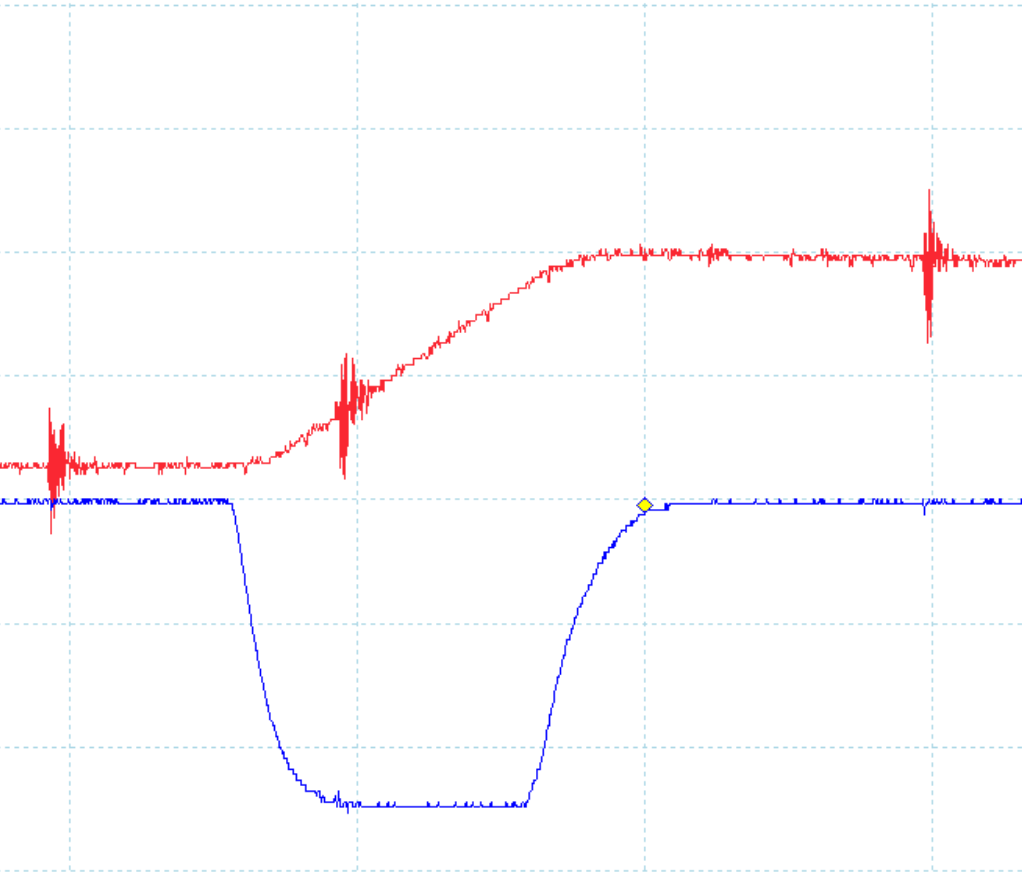
\includegraphics[width=0.38\textwidth]{../preamp/images/screen_interferenza1}
  \caption{\footnotesize Screenshot che mostra il primo fenomeno di interferenza ($0.4\V/div$ e $5\,\si{u\s}/div$).}\label{fig:preamp_interferenza1}%-----------------------------
  \vspace{-35pt} % This removes the white box on the second page
\end{wrapfigure}
\noindent Si vuole infine riportare la presenza di fenomeni di interferenza che sono stati osservati a intervalli irregolari nel corso dell'esperienza: il primo, come mostrato
in Figura~\ref{fig:preamp_interferenza1}, si presenta come una serie di pacchetti d'onda ad alta frequenza
e distanziati $5-10 \,\si{u\s}$, che non ha influenzato particolarmente l'acquisizione
delle misure; la seconda tipologia di interferenza, più rara, verrà invece mostrata in Figura~\ref{fig:shaper_undershoot}, e come si spiegherà nella Sezione~\ref{sec:shaper_pz}, ha disturbato il
segnale al punto da complicare sensibilmente la presa dei dati. Dopo aver controllato con attenzione che tutti i cavi facessero bene contatto, si è giunti alla conclusione che l'origine delle interferenze sia da attribuire ai numerosi dispositivi elettronici presenti
in prossimità del circuito.

\subsection{Analisi del ciruito}\label{sec:preamp_analisi}
Il sistema costituito dal generatore reale (di resistenza
$R_{G}\approx 0.6\kOhm$) e dalle capacità parassite dei cavi in ingresso
($C_{i}\approx 100\,\si{p\farad} $)  presenta una frequenza di taglio di circa
$3 \,\si{M\Hz}$, molto più grande delle frequenze in gioco e pertanto il
generatore può essere assunto ideale.
Risolvendo il circuito del preamplificatore (assumendo ideale l'amplificatore
operazionale) si ottiene la funzione di
trasferimento
\begin{align}\label{eq:preamp_tau}
  \text{A}(s) &= - \frac{1}{R_{1}\,C_{\text{f}}} \, \frac{1}{s+1/\tau_{\text{pre}}}
  &
    \tau_{\text{pre}} &=R_{\text f}\, C_{\text f}=0.154 \pm 0.004\,\si{\milli\second}
\end{align}
da cui si prevede che il circuito si comporterà come un filtro passa basso con
frequenza di taglio
\begin{align}\label{eq:preamp_ft}
  f_{t}&=\frac{1}{2\pi\,\tau_{\text{pre}}}=1.03\pm 0.02\,\si{k\Hz}
  &
    \sigma_{f_{t}}=f_{t}\, \sqrt{
    {\left(\frac{\sigma_{R_{f}}}{R_{f}}\right)}^{2}+
    {\left(\frac{\sigma_{C_{f}}}{C_{f}}\right)}^{2}}
\end{align}
Si prevede inoltre che la risposta del circuito ad un segnale a gradino
sia, per tempi inferiori al periodo $T$, una crescita lineare proporzionale
alla carica $Q_{\text{in}}(t)$ che raggiunge il preamplificatore
\begin{align}\label{eq:preamp_vout}
  V_{\text{out}}& = - \frac{Q_{\inp}(t)}{C_{\text f}} = - \frac{I_{\text{in}}\,}
                  {C_{\text f}}\,t = -\frac{V_{\inp}}{R_{1}}\frac{t}{C_{\text f}}
  &
  \text{per }& 0 < t < T
\end{align}
dove $I_{\text{in}}$ rappresenta la corrente che scorre nella resistenza di
ingresso $R_{1}$.
Per tempi maggiori invece, ci si aspetta una decrescita esponenziale
\begin{align}\label{eq:preamp_vout_exp}
  V_{\text{out}}& = - \frac{Q_{C}}{C_{\text{f}}}\,e^{-\frac{t}{\tau_{\text{pre}}}}=
                  - \frac{I_{\text{in}}\,T}{C_{\text{f}}}\,e^{-\frac{t}{\tau_{\text{pre}}}}
  &
   \text{per }& t> T
\end{align}
dove $Q_{C}$ rappresenta la carica totale accumulata dal preamplificatore.
Si prevede quindi di osservare una tensione massima $V_{\text{max}}=Q_{C}/C_{\text f}$ e, per verificare il funzionamento dell'apparato sperimentale, si confronta
questo valore con una misura diretta della tensione massima rilevata
dall''oscilloscopio: si manda in ingresso un segnale a gradino di periodo
$T=5\,\si{u\s}$ con ampiezza $-1\V$ e si utilizzando i cursori veritcali per
misurare il massimo del segnale in $V_{\text{out}}$ rispetto alla baseline.
Si associa quindi al valore letto l'incertezza sistematica sommata
quadraticamente all'errore di lettura. Sebbene tecnicamente le misure di tensione
siano riferite a due cursori, si sceglie di non considerare il termine $\sqrt 2$ nella
propagazione per evitare sovrastime eccessive dell'errore, in quanto l'oscilloscopio misura
la differenza tra due cursori con una precisione paragonabile a quella della singola misura
\begin{align}\label{eq:v_osc_err}
  V_{\text{max}}^{sp}&=0.344 \pm 0.006 \V
  &
  \sigma_{V_{\text{max}}^{sp}}&=\sqrt{ {\left(\sigma_{L}\times \text{scala}\right)}^{2}+
  {\left(\sigma_{K}\times V_{\text{max}}^{sp}\right)}^{2}}
\end{align}
dove $\sigma_{K}=1.7\%$ rappresenta l'errore di scala fornito dal costruttore (assumendo una distribuzione uniforme) mentre $\sigma_{L}$ rappresenta l'errore di lettura che si attribuisce principalmente alla discretizzazione del segnale e si calcola quindi a partire dalla risoluzione
dell'oscilloscopio $\Delta_{L}= 1/2^{n}$. Nel caso del Picoscope 2204A, vale $n=8\,\text{bits}$ e si ottine equindi $\sigma_{L}=0.002$.
Dalle considerazioni precedenti, invece, segue che la tensione massima attesa vale
\begin{align}
  V_{\text{max}}^{th}&=0.323 \pm 0.012 \V
  &
  \sigma_{V_{\text{max}}^{th}}&=V_{\text{max}}^{th}\,\sqrt{ {\left(\frac{\sigma_{R_{1}}}
                {R_{1}}\right)}^{2}+
 {\left(\frac{\sigma_{C_{\text{f}}}}
                {C_{\text f}}\right)}^{2}+
  {\left(\sigma_{T}\right)}^{2}}
\end{align}
dove, per semplicità, si è trascurato l'errore su $V_{\inp}$ e si assume il valore nominale del generatore. La compatibilità tra le due stime è $\lambda=1.5$, cioè discreta.

\subsection{Verifica della linearità del preamplificatore}\label{sec:preamp_lin}
Si vuole ora verificare la linarità della tensione massima di uscita $V_{\text{out}}$ del preamplificatore
rispetto alla carica in ingresso $Q_{\text{in}}$ (Equazione~\ref{eq:preamp_vout}).
Si modifica quindi la durata dell'impulso del generatore tra $5\,\si{u\s}$ e
$15\,\si{u\s}$ in modo da variare la
quantità di carica iniettata e si misura il massimo del segnale rilevato, sempre
rispetto alla baseline.

\subsubsection{Analisi Dati}\label{sec:pream_lin_an}
Per verificare la linearità del preamplificatore si vuole rappresentare i dati
acquisiti in un grafico ed effettuare un fit, per poi stabilire in base
all'andamento dei residui la validità dell'ipotesi. Alle tensioni (in ordinata)
si associa un errore calcolato come nell'Equazione~\ref{eq:v_osc_err}, considerando quindi
sia la componente sistematica che quella casuale dell'errore, in quanto le misure
sono state acquisite a scale diverse. Questo tuttavia introduce una correlazione
tra i dati di cui il fit non tiene conto e che porta ad una sottostima degli
errori dei parametri. Per quanto riguarda gli errori da associare alla carica
in ingresso $Q_{\text{in},i}=-\frac{V_{\text{in}}}{R_{1} }\,T_{i}$ (in ascissa) la situazione è più complicata. Essi infatti dipendono da
tre fattori: l'errore sulla resistenza $\sigma_{R_{1}}$, sulla tensione
$\sigma_{V_{\text{in}}}$ e sul periodo $\sigma_{T_{i}}$ del segnale in ingresso.
Tuttavia i primi due termini sono costanti per tutte le misure e l'errore
sul periodo è solo sistematico e quindi anch'esso porta un contributo costante.
Segue quindi che gli errori sulla carica sono totalmente correlati e non possono
quindi essere presi in considerazione durante il fit. Si decide allora di
calcolare due interpolazioni: in un primo momento si esegue la regressione lineare
della tensione in uscita $V_{\out}^{\text{max}}$ rispetto al periodo $T$, si ricava il coefficiente
angolare $b$ e si proietta l'errore di scala del periodo
secondo la formula
$\widetilde{\sigma_{b}}=\sqrt{ \sigma_{b,fit}^{2}+b^{2}\, \sigma_{T}^{2}}$. Si esegue
poi il fit di $V_{\text{out}}$ rispetto a $Q_{\text{in}}$, trascurando gli errori
delle ascisse per le considerazioni precedenti. Dal grafico dei residui, che non
dipende dagli errori sistematici, si valuta la linearità del preamplificatore, mentre, per dare una stima all'errore del coefficiente angolare $m$, si sfrutta la
sua relazione con la pendenza $b$ del primo fit
\begin{align}
  m&=\frac{b}{I_{\text{in}}}=\frac{R_{1}}{V_{\text{in}}}\, b
  &
    \sigma_{m} = m\,\sqrt{ {\left(\frac{\widetilde{\sigma_{b}}}{b}\right)}^{2}+
    {\left( \frac{\sigma_{R_{1}}}{R1}\right)}^{2} +
    {\left( \frac{\sigma_{V_{\text{in}}}}{V_{\text{in}}} \right)}^{2}}
\end{align}\label{eq:preamp_lin_eq}%--------------------------------------
In Figura~\ref{fig:preamp_fit_lin} vengono riportati i risultati del secondo fit, il cui grafico
dei residui evidenzia un'ottima distribuzione attorno allo zero e in generale una
buona stima degli errori sulle tensioni, indicata anche dall'errore a posteriori. Anche il chi quadro risulta in ottimo
accordo con l'aspettativa teorica ($\lambda=0.4$). Si conferma quindi l'ipotesi
di linearità della tensione massmia di uscita $V_{\text{out}}^{\text{max}}$ rispetto alla carica
$Q_{\text{in}}$ che raggiunge il preamplificatore.

\noindent Dalla prima interpolazione invece, dopo aver proiettato il contributo di scala
delle ascisse, si ottiene il coefficiente angolare $b=0.057\pm 0.002\V$ e, utilizzando
l'Equazione~\ref{eq:preamp_lin_eq}, si calcola il nuovo errore della pendenza
$m=4.7\pm0.2 \V$. Per l'Equazione~\ref{eq:preamp_vout}, l'inverso di questo coefficiente
angolare corrisponde alla capacità $C_{\text f}$ e infatti la stima $C_{\text{fit}}=0.215\pm0.009 \,\si{n\farad}$ è compatibile con il valore della capacità di feedback ottenuto da una misura diretta col multimetro, anche se
debolmente ($\lambda=2.5$). Tuttavia, l'Equazione~\ref{eq:preamp_vout} prevede anche che
l'intercetta del fit in Figura~\ref{fig:preamp_fit_lin} sia compatibile con lo zero, mentre
risulta $\lambda=5.9$. Si attribuisce questa anomalia alla presenza di errori
sistematici, visto l'ottimo andamento dei residui attorno allo zero (ricordando che essi non
sono affetti da erorri sistematici costanti). Avendo
però acquisito le misure di tensione rispetto alla baseline del segnale di fondo, si esclude la presenza di un errore di offset verticale delle ordinate. Inoltre,
avendo considerato le incertezze di scala delle tensioni nel fit e osservando che
errori di guadagno (costanti) delle ascisse non hanno effetto sull'intercetta,
si attribuisce lo sfasamento dell'intercetta ad un errore di
offset dei periodi. La scelta di attribuire solo un'incertezza sistematica ($\sigma_{T}=3\%$ del valore
nominale), spiegata nella Sezione~\ref{sec:preamp_config_sperim}, va infatti interpretata come un'assunzione
per semplificare i conti, più che un'analisi esaustiva dell'errore.
Si ricorda, infine, che avendo considerato gli errori sistematici
delle tensioni nei fit, si è introdotta una correlazione che porta ad una
sottostima degli errori e quindi a compatibilità peggiori. Si decide allora
di confermare l'ipotesi di linearità del preamplificatore, ma si ritiene
l'analisi svolta insufficiente per confermare la validità dell'Equazione~\ref{eq:preamp_vout}.
%------------------------------------
\begin{figure}[h]
\centering
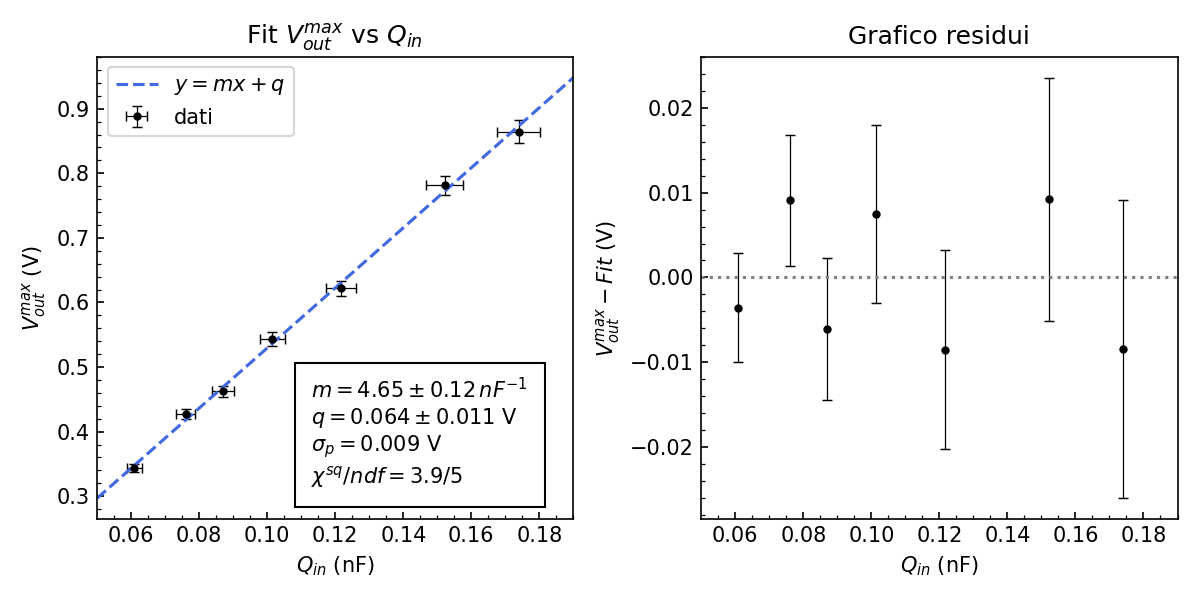
\includegraphics[width=0.8\textwidth]{../preamp/images/fit_lin}
\caption{\footnotesize A sinistra si mostrano i dati sperimentali e il fit della tensione massima in uscita rispetto alla carica in ingresso. Gli errori delle ascisse vengono riportati
  a scopo dimostrativo ma non vengono considerati nel fit, come spiegato. Le incertezze sui parametri
  mostrate sono quelle ottenute dall'interpolazione. Inoltre, a destra, viene riportato il grafico dei residui.}\label{fig:preamp_fit_lin}
\end{figure}
%------------------------------------

\subsection{Tempo Caratteristico del Preamplificatore}\label{sec:preamp_ft}
In questa sezione ci si concentra sulla fase di scarica del segnale. Con l'obiettivo di stimare
il tempo caratteristico del preamplificatore a partire da un fit esponenziale (Equazione~\ref{eq:preamp_vout_exp}) e
da uno lineare, si manda in ingresso un onda quadra di periodo\footnote{Si segnala una svista in fase di acquisizione dati per cui il periodo dell'onda quadrata è stato impostato a $50\us$, diversamente da quanto detto.}  $T=5\,\si{u\s}$ e ampiezza $1\V$, e si misura la tensione in uscita $V_{\text{out}}$ in corrispondenza di istanti di tempo $t$ diversi.

\subsubsection{Analisi Dati}\label{sec:preamp_ft_analisi}
Alle misure di tensione viene associato l'erore di lettura dell'oscilloscopio,
analogamente a quanto svolto nella sezione precedente. All'istante di tempo
$t$ si associa invece un errore (massimo) di lettura pari a $1/10$ dei $secondi/divisione$ corrisponendi alla scala selezionata. Per evitare di
sovrastimare l'errore si assume ora una distribuzione triangolare, ottenendo quindi un errore di lettura di $\sigma_{L}=0.04\,\text{div}$. L'errore di guadagno sui
tempi fornito dal costruttore è dello $0.01\%$ e si assume quindi trascurabile.
Gli errori relativi dei tempi così calcolati sono generalmente di un ordine di grandezza inferiore rispetto alle incertezze relative delle tensioni. Si decide quindi
di effettuare il fit esponenziale $y=a+b \exp(t\,c)$ considerando solo gli errori delle ordinate. I risultati dell'interpolazione e una simulazione
LTspice del circuito sono riportati in
Figura~\ref{fig:preamp_fit_exp_lin}: dal grafico dei residui si evidenzia un ottimo andamento
attorno allo zero ma una leggera sovrastima degli errori, indicata anche
dalla deviazione standard a posteriori e dal chi quadro eccessivamente basso.
L'inverso del parametro $c$ rappresenta la prima stima sperimentale del
tempo caratteristico $\tau_{\text f,\text{exp}}= 0.16\pm 0.01\,\si{m\s}$, in ottima compatibilità con l'aspettativa teorica calcolata nell'Equazione~\ref{eq:preamp_tau} ($\lambda=0.2$).
Anche il parametro $a$ risulta perfettamente compatibile con lo zero
($\lambda=0.6$). Ci si aspetta infine che il parametro $b$ corrisponda
alla carica totale scalata dall'inverso della capacità di feedback
\begin{align}
  b_{th}=-\frac{Q_{C}}{C_{\text f}}& =-\frac{V_{\text{in}}\,T}{R_{1}\, C_{\text{f}}}=3.21 \pm 0.10 \V
  &
    \sigma_{b_{th}}& = b_{th}\,
                     \sqrt{{\left(\frac{\sigma_{V_{\text{in}}}}{V_{\text{in}}}\right)}^{2}+
                     {\left(\frac{\sigma_{R_{1}}}{R_{1}}\right)}^{2}+ {\left(\frac{\sigma_{C_{\text f}}}{C_{\text f}}\right)}^{2}+
                     \sigma_{T}^{2}}
\end{align}
dove $V_{\text{in}}= 0.99\pm 0.02 \V$ viene misurato direttamente con l'oscilloscopio. Confrontando $b_{th}$ col valore
%------------------------------------
\begin{figure}[h]
\centering
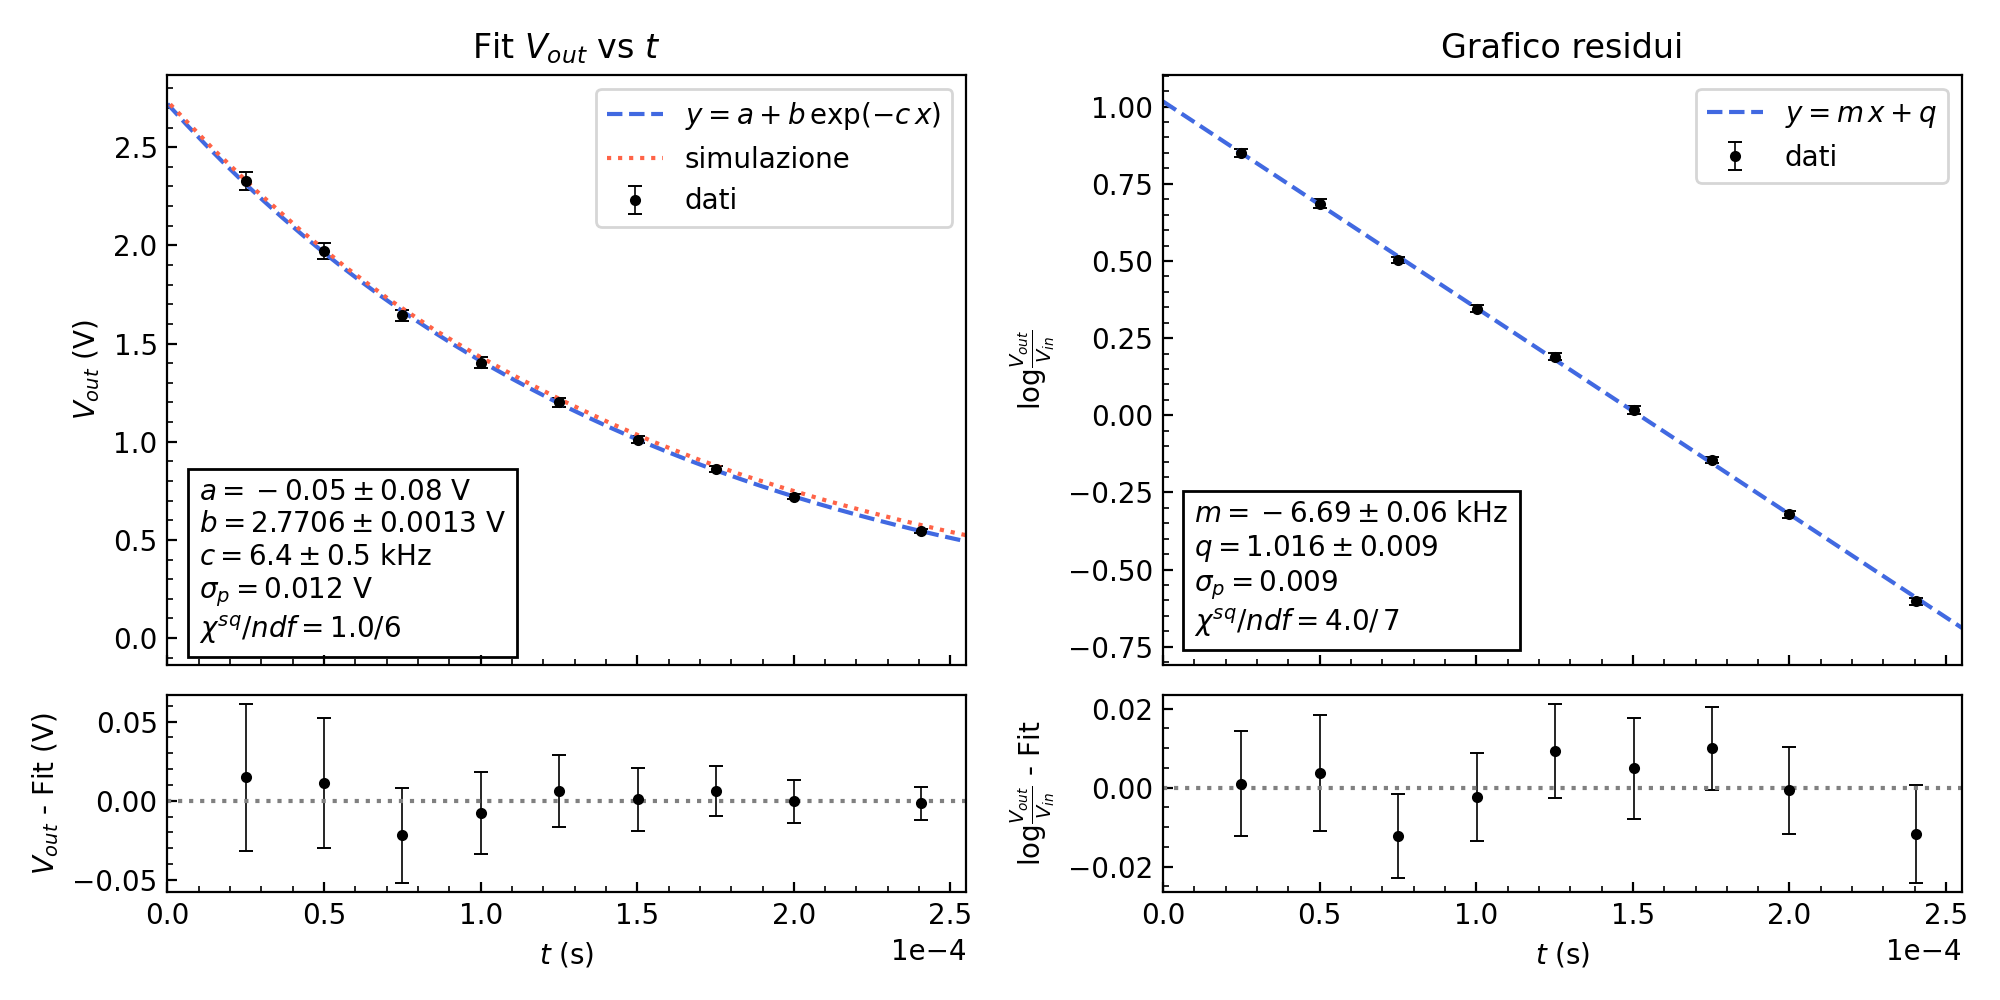
\includegraphics[width=0.9\textwidth]{../preamp/images/fit_exp_lin}
\caption{\footnotesize A sinistra si mostrano il fit esponenziale e la
  simulazione ottenuta con LTspice mentre a destra viene riportata l'interpolazione lineare. Sotto entrambi i grafici vengono mostrati anche gli andamenti dei residui.}\label{fig:preamp_fit_exp_lin}
\end{figure}
%------------------------------------
\noindent ottenuto dal fit si
riscontra che tali valori sono incompatibili ($\lambda=4.4$). Visto il buon
accordo dei dati con la simulazione LTspice, si attribuisce questa
discrepanza alla correlazione introdotta considerando gli errori sistematici
sulle tensioni, che porta ad una sottostima dell'errore dei parametri.
\noindent Si vuole ora ottenere una nuova stima del tempo caratteristico a partire da
un fit lineare, considerato più robusto rispetto all'interpolazione
non lineare. Dopo aver diviso entrambi i membri per $V_{\text{in}}$ in modo da rendere
adimensionale l'argomento del logaritmo, si linearizza l'Equazione~\ref{eq:preamp_vout_exp}
ottenendo la relazione
\begin{align}
  y & = \log{\left|\frac{V_{\text{out}}}{V_{\text{in}}}\right|} = -\frac{t}{\tau}+\log{\left(\frac{T}{R_{1}C_{\text f}}\right)}
  &
    \sigma_{y}&= |y| \sqrt{{\left(\frac{\sigma_{L}\times \text{scala}_{in}}{V_{\text{in}}}\right)}^{2}+
    {\left(\frac{\sigma_{L}\times \text{scala}_{out}}{V_{\text{out}}}\right)}^{2}}
\end{align}
dove nel calcolo dell'errore sulle y si sono trascurati i contributi dell'errore di scala
di $V_{\text{in}}$ e $V_{\text{out}}$ in quanto, per le proprietà del logaritmo, si trasferiscono sull'intercetta.
I risultati del fit lineare sono riportati in Figura~\ref{fig:preamp_fit_exp_lin}, da cui si
osserva una buona distribuzione dei residui attorno allo zero e una
discreta stima dell'errore. Dall'inverso del coefficente angolare si ricava
la seconda stima sperimentale del tempo caratteristico $\tau_{\text{lin}}=0.1496\pm0.0013 \,\si{m\s}$. Tale valore risulta compatibile con la stima
ottenuta dal fit esponenziale ($\lambda=1.0$) ed è in ottimo accordo anche con il valore
ricavato dall'Equazione~\ref{eq:preamp_tau} ($\lambda=1.0$). Si preferisce la stima
ottenuta dal fit lineare in quanto meno affetta da errori sistematici.

\subsection{Risposta in frequenza del Preamplificatore}\label{sec:preamp_bode}
In questa sezione si approfondisce la risposta in frequenza del preamplificatore, registrando il massimo della tensione in uscita
$V_{\text{out}}$ per segnali sinusoidali di ampiezza $1\V$
e di frequenze comprese tra $10\,\si{\Hz}$ e $100\,\si{k\Hz}$. Dal grafico di Bode si ottiene poi una stima della
frequenza di taglio del circuito.

\subsubsection{Analisi Dati}\label{sec:bode_analisi}
Per realizzare il grafico di Bode (Figura~\ref{fig:preamp_fit_bode}) si esprime la funzione di trasferimento
in decibel
\begin{align}
  H(dB) &= 20\log_{10}{\left(\frac{V_{\text{out}}}{V_{\text{in}}}\right)}
  &
    \sigma_{H}(dB) = 20\,\log_{10}{(e)}\,\sqrt{{\left(\frac{\sigma_{L}\times \text{scala}_{in}}{V_{\text{in}}}\right)}^{2}+
    {\left(\frac{\sigma_{L}\times \text{scala}_{out}}{V_{\text{out}}}\right)}^{2}}
\end{align}
%------------------------------------
\begin{figure}[h]
\centering
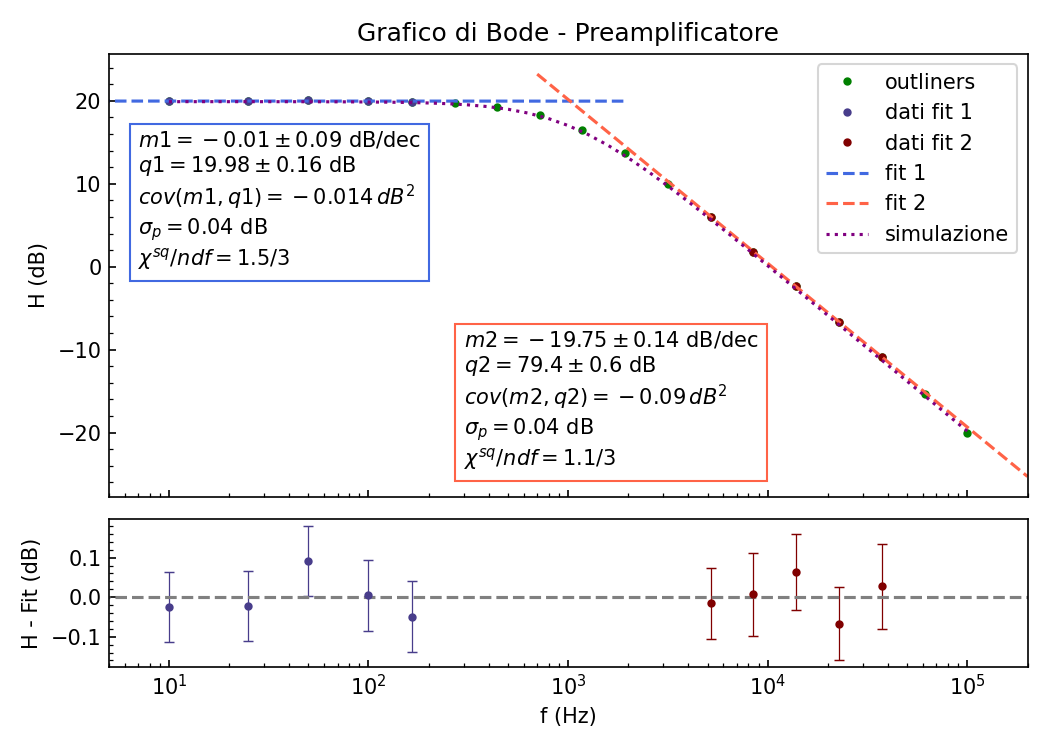
\includegraphics[width=0.7\textwidth]{../preamp/images/fit_bode}
\caption{\footnotesize Grafico di Bode del preamplificatore. Oltre ai dati sperimentali, si mostrano le due interpolazioni coi relativi
grafici dei residui e outliners (in verde). Vengono presentati anche i risultati di una simulazione (in viola).}\label{fig:preamp_fit_bode}
\end{figure}
%------------------------------------
Le frequenze vengono mostrate in scala logaritmica e si assume che la
loro incertezza sia trascurabile.
 Nella Figura~\ref{fig:preamp_fit_bode} si mostrano anche i
risultati di una simulazione del circuito che evidenzia un buon accordo per tutte le frequenze sia con i dati sperimentali che con le previsione teoriche: come spiegato in Sezione~\ref{sec:preamp_analisi} il circuito si comporta come un filtro passo basso e infatti per frequenze inferiori a $\approx 1\kHz$ la funzione di trasferimento
è approssimabile ad una retta di pendenza compatibile con lo zero (rappresentata in blu in Figura~\ref{fig:preamp_fit_bode}). A frequenze più alte invece,
la funzione di trasferimento decresce come una retta con pendenza
di circa $20 \,dB$ (in rosso).
\noindent L'intersezione tra le due rette fornisce una stima
della frequenza di taglio del circuito
\begin{align}
  f_{t}&=\frac{q_{1}-q_{2}}{m_{2}-m_{1}}=1.02\pm 0.03\,\si{k\Hz},
  &
    \sigma_{f_{t}}&= f_{t}\,\sqrt{  \frac{\sigma_{q_{1}}^{2}+\sigma_{q_{2}}^{2}}{{(q_{1}-q_{2})}^{2} } +
                    \frac{\sigma_{m_{1}}^{2}+\sigma_{m_{2}}^{2}}{{(m_{2}-m_{1})}^{2} } +
                    2\frac{\text{cov}(q_{1},m_{1})+\text{cov}(q_{2},m_{2})}{(q_{1}-q_{2})(m_{2}-m_{1})} }
\end{align}
compatibile sia con l'aspettativa teorica calcolata in Equazione~\ref{eq:preamp_ft} ($\lambda=0.2$) che con la frequenza ottenibile dalla stima del tempo caratteristico
della sezione precedente $f_{t,\text{lin}}= 1.064\pm 0.010\kHz$ (in questo caso vale $\lambda=1.5$).


\section{Shaper CR-RC}\label{sec:shaper}
In questa sezione si realizza il secondo modulo della catena elettronica: si tratta di un circuito (detto shaper) per modificare la forma del
segnale in uscita dal preamplificatore (rendendolo simile ad una gaussiana) e
per ridurne la durata. Si vuole in particolare evitare che si verifichi il fenomeno di ``pile up'' del segnale, che si manifesta in situazioni di alte
frequenze di acquisizione in cui i segnali possono sovrapporsi e compromettere così l'informazione da acquisire.
Si studia inoltre la risposta in frequenza dello shaper e infine si
osserva e corregge l'effetto di Pole-Zero.

%------------------------------------------------
%	Configurazione Sperimentale
%------------------------------------------------

\subsection{Configurazione Sperimentale}\label{sec:shaper_config}
\begin{wrapfigure}{r}{0.5\textwidth}
  \centering
  \begin{circuitikz}[scale=0.7, transform shape, use fpu reciprocal]
     \draw(0,0) node[ground]{}
      (0,2) to[american voltage source,l=$V_{gen}$](0,0);
      \draw(0,2)-- (1,2) to[C,l_=$C_{sh1}$,font=\boldmath] (4,2)
          (4,2) to[R,l=$R_{sh1}$,font=\boldmath] (4,0) to (4,0) node[ground]{};
      \draw(6,2.5) node[op amp] (OA2){$OA_{2}$}
        (OA2.+)-- (4,2)
        (OA2.-)-- (4.5,3)-- (4.5,4)-- (7.5,4)-- (7.5,2.5)
        (OA2.out)-- (8,2.5) to[R,l=$R_{sh2}$,font=\boldmath] (10,2.5)
          (10,2.5) to[C,l_=$C_{sh2}$,font=\boldmath] (10,1) node[ground]{}
       (10,2.5) to[short,-*,l=$V_{out}$,font=\boldmath] (11,2.5);
    \end{circuitikz}
  \caption{\footnotesize Schema a variabili concentrate del circuito shaper $CR-RC$.}\label{fig:shaper-circuito}
\end{wrapfigure}
Si assembla il circuito in Figura~\ref{fig:shaper-circuito} utilizzando due capacità uguali
$C_{\text{sh1}}$, $C_{\text{sh2}}$ e due resistenze
uguali $R_{\text{sh1}}$,$R_{\text{sh2}}$, i cui valori,
misurati col multimetro, vengono riportati nella Tabella~\ref{tab:shaper_misure}.
Si usa il secondo amplificatore operazionale incluso nello stesso integrato
TL082 utilizzato per il preamplificatore come buffer per disaccoppiare i due stadi
$C_{\text{sh1}}R_{\text{sh1}}-R_{\text{sh2}},C_{\text{sh2}}$. In un primo momento si inserisce in
ingresso un'onda quadra di bassa frequenza per simulare un preamplificatore
ideale che mantiene il segnale per un tempo indefinito e, dopo aver confrontato la risposta del circuito con le aspettative
teoriche e le simulazioni, si inserisce come ingresso dello shaper
l'output del preamplificatore operazionale.
\begin{table}[h]
\centering
\setlength{\tabcolsep}{10pt}
\begin{tabular}{ |c|c|c|  }
\hline
\multicolumn{3}{|c|}{Misure dirette dei componenti del circuito} \\
\hline
Label      & Valore & F.S.\\
\hline
$R_{\text{sh1}}$ & $100.2 \pm 0.5\kOhm$ & $200\kOhm$ \\
$R_{\text{sh2}}$ & $100.1 \pm 0.5\kOhm$ & $200\kOhm$ \\
$C_{\text{sh1}}$ & $0.102 \pm 0.003\nF$ &$2\nF$ \\
$C_{\text{sh2}}$ & $0.103 \pm 0.003\nF$ &$2\nF$ \\
\hline
\end{tabular}
\caption{\footnotesize Si mostrano in tabella i valori e le incertezze delle componenti usate
  per la realizzazione dello shaper, misurati con il multimetro Tenma. È stato riportato anche il fondo scala usato.}\label{tab:shaper_misure}
\end{table}

%------------------------------------------------
%	Analisi del circuito
%------------------------------------------------

\subsection{Analisi del circuito}\label{sec:shaper_analisi}
Dai valori riportati in Tabella~\ref{tab:shaper_misure} si ottengono due
stime dello shaping time $\tau_{sh1}=10.2\pm 0.3 \us$ e
$\tau_{sh2}=10.3\pm 0.3 \us$.
Vista l'ottima compatibilità, si procede col calcolare la media pesata  tra i due valori $\langle \tau_{sh}\rangle = 10.26\pm 0.14 \us$.
Assumendo ideale l'amplificatore operazionale e risolvendo il circuito
nell'ipotesi $\tau_{sh1}=\tau_{sh2}=\tau_{sh}$, si ottiene le funzione di trasferimento
\begin{align}
  A(s)=\frac{1}{\tau_{sh}}\,\frac{s}{{(s+\frac{1}{\tau_{sh}})}^{2}}
\end{align}
da cui si prevede che la risposta a un segnale di ingresso a gradino sia
\begin{align}
  V_{\out}=\frac{V_{\inp}}{\tau_{\sh}}\, t\, e^{-\frac{t}{\tau_{\sh}}}
\end{align}
Essa presenta una forma simile ad una gaussiana di larghezza proporzionale allo shaping time
$\tau_{\sh}$ e ha massimo
\begin{align}
  V_{\out}^{\text{max}}& =V_{\inp}/e
  &
    t_{\text{max}}&= \tau_{sh}
\end{align}
Dalla funzione di trasferimento si deduce inoltre che il circuito si comporta
come un derivatore
\begin{wrapfigure}{r}{0.5\textwidth}
  \centering
  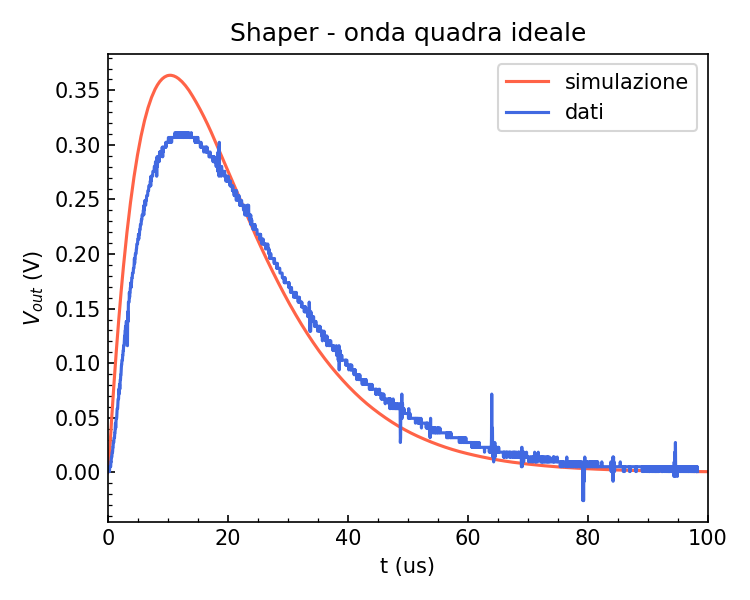
\includegraphics[width=0.48\textwidth]{../shaper/images/grafico_esp}
  \caption{\footnotesize{Risposta dello shaper ad un'onda quadra ideale.}}
\label{fig:shaper_id}%-----------------------------
\end{wrapfigure}
\noindent a basse frequenze e che, dopo una breve regione di midband, si comporta come
un integatore a frequenze alte.
Per verificare la corretta configurazione dell'apparato sperimentale si acquisicono
delle prime misure esplorative: si imposta il generatore in modo da erogare un'onda quadra
di frequenza $100\Hz$ e ampiezza $1\V$ per simulare un preamplificatore ideale. Utilizzando
i cursori di tensione e di tempo dell'oscilloscopio, si misura il massimo della tensione (rispetto alla baseline) in uscita, l'ampiezza dell'onda quadra in ingresso e lo shaping time.
I risultati delle misure e le aspettative teoriche sono riportate in Tabella~\ref{tab:shaper_misure_osc}, da cui si evidenzia una forte incompatibilità sia per
la tensione massima che per lo shaping time. Si attribuisce questa discrepanza alla non idealità dei componenti del circuito e alla presenza di capacità parassite dovute ai cavi e alla breadboard che portano ad una sottostima del tempo caratteristico. Questa anomalia risulta ancora più
evidente dal grafico in Figura~\ref{fig:shaper_id}, in cui viene confrontato il segnale rilevato
dall'oscilloscopio con la simulazione LTspice.

\begin{table}[h]
\centering
\setlength{\tabcolsep}{10pt}
\begin{tabular}{ |c|c|c|  }
\hline
\multicolumn{3}{|c|}{Misure oscilloscopio} \\
\hline
\multicolumn{3}{|c|}{$V_{\inp,\text{sp}}= 0.98 \pm 0.02\V$} \\
\hline
Misura      & Aspetattiva & Compatibilità\\
$V_{\out,\text{sp}}^{\text{max}}= 0.315\pm 0.006\V$    & $V_{\out,\text{th}}^{\text{max}}= 0.362\pm 0.007\V$  & $\lambda=5.0$\\
$\tau_{\sh,\text{sp}}= 11.7 \pm 0.4\us$  & $\tau_{\sh,\text{th}}= 10.3\pm 0.3\us$ & $\lambda=12.8$\\
\hline
\end{tabular}
\caption{\footnotesize{Si mostrano in tabella i valori e le incertezze delle misure effettuate con l'oscilloscopio. In particolare si riporta la tensione massima sperimentale $V_{\out,\text{sp}}^{\text{max}}$, lo shaping time $\tau_{\sh,\text{th}}$ e la misura dell'ampiezza
  dell'onda quadra in ingresso. Si riportano anche le aspettative teoriche e si calcola la compatibilità.}}\label{tab:shaper_misure_osc}
\end{table}

%------------------------------------------------
%	Risposta in frequenza dello shaper
%------------------------------------------------

\subsection{Risposta in frequenza dello Shaper}\label{sec:shaper_bode}
In questa sezione si studia la risposta del circuito a segnali sinusoidali di ampiezza
$1\V$ e frequenze comprese tra $0.1\kHz$ e $100\kHz$. Si registrano quindi per ogni
frequenza campionata le tensioni di ingresso e di uscita utilizzando i cursori verticali
dell'oscilloscopio. Infine, si realizza il grafico di Bode e da esso si stima la frequenza relativa al polo della funzione di trasferimento.

\subsubsection{Analisi Dati}\label{sec:shaper_bode_analisi}

Per il calcolo della funzione di trasferimento e per le considerazioni sulla sua incertezza
si rimanda alla Sezione~\ref{sec:preamp_bode}. Si mostra in Figura~\ref{fig:shaper_bode} il grafico di Bode
confrontato con una simulazione. Si nota subito come il circuito si comporti come previsto
nella Sezione~\ref{sec:shaper_analisi}: per basse frequenze funziona come derivatore e presenta
una regione ad alta frequenza in cui integra. Tuttavia, sono evidenti numerose discrepanze con la simulazione, soprattuto a basse e alte frequenze. Questo non sorprende considerando gli scarsi
risultati già ottenuti nella sezione precedente e soprattutto osservando l'ampio range di
frequenze analizzato.
In Figura~\ref{fig:shaper_bode} vengono riportate anche due interpolazioni lineari: una per la
regione di derivazione (in blu) e una per quella di integrazione (in rosso).
L'intersezione delle due rette fornisce una stima della frequenza relativa
al polo doppio della funzione di trasferimento dello shaper $f_{\text{fit}}=12.3\pm 0.3 \kHz$,
compatibile con l'aspettativa $f_{\text{sp}}=13.6\pm 0.5\kHz$, ottenuta utilizzando la stima sperimentale
dello shaping time riportata in Tabella~\ref{tab:shaper_misure_osc} ($\lambda=2.3$). Risulta invece incompatibile ($\lambda=8.4$) con la frequenza
$f_{\text{th}}=15.5\pm 0.2\kHz$, ricavata a partire dallo shaping time teorico.
\begin{figure}[h]
\centering
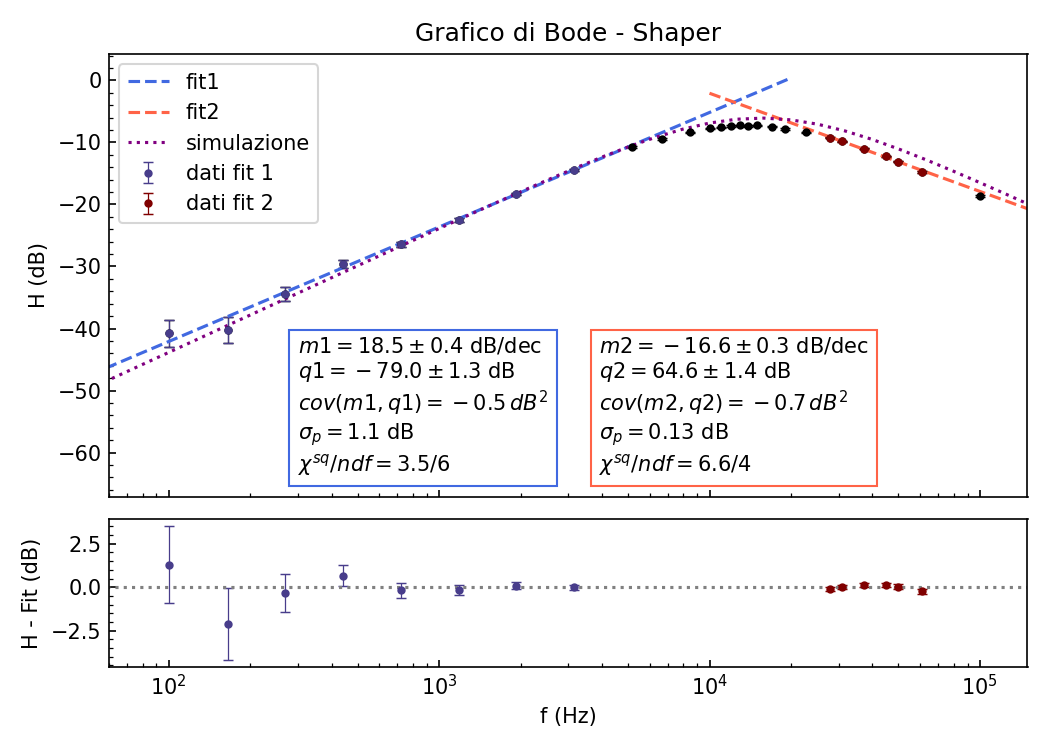
\includegraphics[width=0.8\textwidth]{../shaper/images/fit_bode}
\caption{\footnotesize Grafico di Bode dello shaper $CR-RC$ confrontato con la simulazione LTspice. In basso vengono mostrati i residui delle due interpolazioni lineari.}\label{fig:shaper_bode}
\end{figure}

%------------------------------------
%------------------------------------------------
%	Shaper con Pole-Zero
%------------------------------------------------

\subsection{Shaper con compensazione Pole-Zero}\label{sec:shaper_pz}

Si mette ora in input allo shaper l'output del preamplificatore: in questo modo non si ha più
un'onda quadra ideale in ingresso, ma un segnale che cresce linearmente e caratterizzato da
una discesa lenta. Si osserva quindi il fenomeno di undershoot, per cui la tensione prima
di raggiungere asintoticamente la baseline diventa negativa fino a raggiungere
il minimo
$V_{\text{undershoot}}\approx-25\,\si{m\volt}$, per poi risalire
lentamente. Questo vanifica parzialmente l'effetto di riduzione della durata
del segnale dello shaper e quindi si cerca di rimediare tramite
il metodo di compensazione Pole-Zero: aggiungendo una resistenza $R_{\text{pz}}$ in parallelo al condensatore $C_{\sh 1}$, il segnale che
arriva all'ingresso dell'$RC$ è dato da
\begin{align}
  V_{1}(s)&=\frac{V_{\inp}}{s+\frac{1}{\tau_{\text{pre}}}}\frac{s+\frac{1}{\tau_{\text{pz}}}}{s+\frac{1}{\tau_{\parallel}}}
  &
    \text{con }& \begin{cases}
      \tau_{\text{pz}}=R_{\text{pz}}\,C_{\text{sh1}}\\
      \tau_{\parallel}=R_{\parallel}\,C_{\text{sh1}}=\left(\frac{1}{R_{1}}+\frac{1}{R_{\text pz}}\right)^{-1}\,C_{\text{sh1}}
    \end{cases}
\end{align}
Scegliendo la resistenza di Pole-Zero tale che valga la relazione $\tau_{\text{pz}}=\tau_{\text{pre}}$, si annulla l'effetto del polo del preamplificatore,
responsabile del fenomeno di undershoot. Deve quindi valere $R_{\text{pz}}=1.51\pm 0.06\MOhm$ e, osservando che
tale valore è molto più grande delle resitenze $R_{\sh 1}$ e $R_{\sh2}$, segue che $\tau_{\parallel}\approx \tau_{\sh 1}$
e si ottiene approssimativamente lo stesso polo del circuito $CR$ non modificato. Si aggiungono quindi al circuito due resistenze in serie in modo
da ottenere la resistenza equivalente
\begin{align}
  R_{\text{pz,sp}}&= (0.558\pm0.002)\MOhm + (1.009\pm0.005)\MOhm = (1.567\pm 0.006) \MOhm
\end{align}
che presenta un'ottima compatibilità col valore richiesto ($\lambda=0.9$).
In Figura~\ref{fig:shaper_undershoot} viene mostrato il segnale di uscita dell'oscilloscopio prima e
dopo la correzione di Pole-Zero. Si mostra anche il fenomeno di interferenza
anticipato nella Sezione~\ref{sec:preamp_config_sperim} e che ha dominato questa parte dell'esperienza.
Il segnale risulta infatti visibilmente ``sporco'', complice anche il fatto
che le tensioni in gioco sono prossime ai limiti imposti dalla precisione
del Picoscope. Si nota comunque un discreto accordo con le simulazioni e
dopo $10\, \tau_{\text{sh1}}$ la tensione risulta compatibile con la baseline, confermando, per quanto possibile date le circostanze, una
corretta compensazione di Pole-Zero.
%------------------------------------
\begin{figure}[h]
\centering
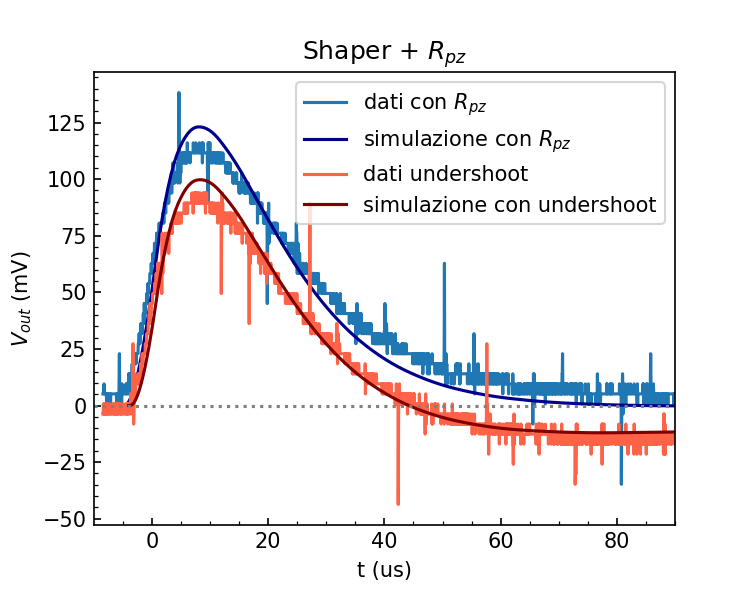
\includegraphics[width=0.6\textwidth]{../shaper/images/undershoot}
\caption{\footnotesize{Si mostrano in grafico le simulazioni e i segnali rilevati dall'oscilloscopio in configurazione con undershoot e con compensazione di Pole-Zero. Si osserva anche il fenomeno di forte interferenza che ha complicato l'acquisizione delle misure in quest'ultima sezione relativa allo shaper.}}\label{fig:shaper_undershoot}
\end{figure}


\section{Catena Elettronica Completa}\label{sec:catena}
In questa sezione si assembla un circuito amplificatore con l'obiettivo di portare l'output dello shaper
entro i range tipici dei sistemi di acquisizione dati (DAQ), generalmente tra i $2\V$ e i $5\V$.
Essendo già positivo il segnale in uscita dallo shaper, si assembla il circuito in configurazione non invertente,
come mostrato nel terzo e ultimo modulo della catena rappresentata in Figura~\ref{fig:circ_tot}. Dopo aver calcolato gli opportuni valori delle resistenze $R_{1a}$ e $R_{2a}$,
si connette l'amplificatore al resto della catena elettronica e se ne studia la linearità e la risposta in
frequenza.

\subsection{Configurazione sperimentale e prime misure}\label{sec:catena_config}
Per capire con quali resistenze costruire il circuito, si manda in ingresso
al preamplificatore un'onda quadra di periodio $15\us$ e si registra la
tensione massima di output dello shaper $V_{\text{sh}}^{\text{max}}=0.290\pm 0.006\V$.
Data la funzione di trasferimento di un amplificatore non invertente
\begin{align}
  A(s)=1+\frac{R_{a2}}{R_{a1}}
\end{align}
segue che, per ottenere una tensione di $2\V$ in uscita dalla catena elettronica, il rapporto tra le due resistenze deve valere $R_{a2}/R_{a1}=5.9$. Con le resistenze a disposizione si sceglie
$R_{a1}=32.80\pm 0.2\kOhm$ mentre la resitenza di feedbeck si realizza mettendo in serie
due resistori di impedenza equivalente
\begin{align}
  R_{a2}= (67.9\pm 0.3)\kOhm + (120.6 \pm 0.6)\kOhm = (188.5 \pm 0.7)\kOhm
\end{align}
Si prevede quindi un'amplificazione $A=6.75\pm 0.06$, debolmente compatibile con quella richiesta ($\lambda=2.5$). Per verificare la correttezza delle ipotesi si manda in ingresso all'amplificatore invertente appena
assemblato un'onda sinusoidale di frequenza $1\kHz$ e ampiezza $1\V$ e
si misura con l'oscilloscopio la risposta del circuito. Successivamente, si
inserisce il segnale di uscita dello shaper come input dell'amplificatore non
invertente e si misura nuovamente la risposta del circuito. I valori acquisiti e le compatibilità con le aspettative teoriche vengono riportati in
Tabella~\ref{tab:amp_misure}, la quale evidenzia un'ottimo accordo e conferma quindi
la correttezza dell'apparato sperimentale.
\begin{table}[h]
\renewcommand{\arraystretch}{1.6}
\centering
\setlength{\tabcolsep}{10pt}
\begin{tabular}{ |cccc| }
\hline
\multicolumn{4}{|c|}{Preamplificatore - onda sinusoidale} \\
$V_{\inp}^{\text{max}}=0.99\pm 0.02\V$ & $V_{\out}^{\text{max}}=6.67\pm 0.12\V$ & $A_{\text{amp}}=6.8\pm 0.2$ & $ \lambda_{A}=0.14$\\
\hline
\multicolumn{4}{|c|}{Catena elettronica - onda quadra} \\
$V_{\inp}^{\text{max}}=-1.00\pm 0.02\V$ & $V_{\out}^{\text{max}}=2.08\pm 0.04\V$ &$|A_{\text{catena}}|=2.09\pm 0.06$ & $\lambda_{V_{\out}}=1.9$ \\
\hline
\end{tabular}
\caption{\footnotesize Si mostrano le misure acquisite con l'oscilloscopio in due configurazioni: onda sinusoidale in input al preamplifcatore e onda onda quadra in  ingresso alla catena completa. Si calcolano inoltre le compatibilità tra l'amplificazione prevista e quella osservata (nel primo caso) e tra la tensione in output misurata e il valore richiesto di $2\V$ (nel secondo caso).}\label{tab:amp_misure}
\end{table}
%-------------------------------------


\subsection{Analisi del circuito }\label{sec:catena_analisi}
La catena elettronica completa, mostrata in Figura~\ref{fig:circ_tot}, ha come funzione di
trasferimento il prodotto delle funzioni di trasferimento dei tre moduli che
la compongono
\begin{align}
  A(s)= A_{\text{pre}}(s) \, A_{\text{sh}}(s) \, A_{\text{ampl}}(s) = \left(-
  \frac{\frac{1}{R_{1}C_{\text{f}}}}{s+\frac{1}{\tau_{\text{pre}}}}\right) \, \left(\frac{1}{\tau_{\text{sh}}}\,\frac{s+\frac{1}{\tau_{\text{pz}}}}{(s+\frac{1}{\tau_{\text{sh}}})(s+\frac{1}{\tau_{\parallel}})}\right) \,\left(1+\frac{R_{a2}}{R_{a1}}\right)
\end{align}
Avendo scelto la resistenza $R_{\text{pz}}$ tale che $\tau_{\text{pz}} = \tau_{\text{pre}}$ ed essendo essa molto più grande delle resitenze dello shaper la funzione di trasferimento assume la forma semplificata
\begin{align}
  A(s)=- \frac{1}{R_{1}\,C_{\text{f}}\, \tau_{\text{sh}}} \,\,
  \frac{1+\frac{R_{2a}}{R_{1a}}}{\left(s+\frac{1}{\tau_{\text{sh}}}\right)^{2}}
\end{align}
La funzione di trasferimento è quindi caratterizzata dall'assenza di zeri e
dalla presenza dello stesso polo doppio trovato nello shaper. La catena si comporta
quindi come un filtro passa basso: per frequenze piccole il grafico di Bode presenterà un andamento costante, mentre per frequenze elevate si prevede
una decrescita lineare di $40\,dB/dec$. La frequenza di taglio attesa è la
stessa calcolata nella Sezione~\ref{sec:shaper_bode_analisi}, ovvero $f_{t}= 15.5\pm 0.2\kHz$.

\subsection{Linearità della Catena Elettronica}\label{sec:catena_lin}
Si vuole ora verificare la linearità del massimo del segnale di uscita $V_{\out}^{\text{max}}$ della catena elettronica rispetto alla quantità di carica iniettata nel preamplificatore $Q_{\text{in}}$. Si modifica quindi la
durata dell'impulso del generatore tra $5\us$ e $15\us$ e si misura con
l'oscilloscopio il massimo del segnale rilevato.

\subsubsection{Analisi dati }\label{sec:catena_lin_analisi}
Per l'analisi dati si procede esattamente come in Sezione~\ref{sec:preamp_lin}: si calcola la
quantità di carica $Q_{\inp}$ per ogni valore di $T$ utilizzato e, a causa
della correlazione totale degli errori sulle cariche, si effettua il fit senza prendere in considerazione gli errori sulle ordinate. A differenza di
quanto svolto in precedenza però, si sceglie di non correggere l'errore sulla pendenza effettuando un primo fit rispetto ai periodi. In questa sezione si preferisce infatti concetrarsi solo sulla verifica della linearità e quindi
sul grafico dei residui, che non è influenzato dalla presenza di errori di
scala costanti. I risultati del fit vengono mostrati in Figura~\ref{fig:catena_fit_lin}, che evidenzia una buona distribuzione dei residui attorno allo zero e una leggera
sovrastima degli errori per i periodi più grandi. Il chi quadro presenta un'ottima
compatibilità col valore atteso ($\lambda=0.11$). Si conferma quindi l'ipotesi di linearità
della catena elettronica.
%------------------------------------
\begin{figure}[h]
\centering
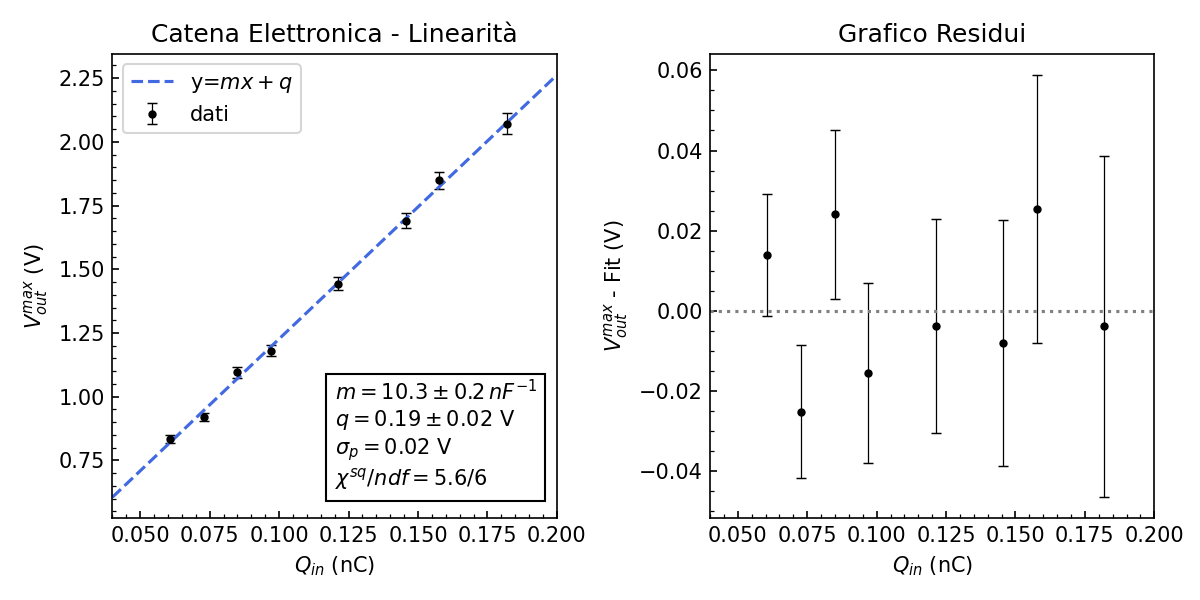
\includegraphics[width=1\textwidth]{../ampli/images/fit_lin}
\caption{\footnotesize A sinistra si mostrano le coppie $(V_{\text{out}}^{\text{max}}, Q_{\text{in}})_{i}$ e la retta interpolante. A destra, viene riportato il grafico dei residui.}\label{fig:catena_fit_lin}
\end{figure}
%------------------------------------

\subsection{Risposta in frequenza della Catena Elettronica}\label{sec:catena_bode}
Si vuole infine approfondire la risposta in frequenza della catena elettronica. Si acquisce quindi il massimo della tensione in uscita $V_{\out}^{\text{max}}$
per segnali sinusoidali di frequenza variabile tra $10 \Hz$ e $100\kHz$. Si rappresentano quindi i dati in un grafico di Bode e si stima la frequenza di taglio della catena a partire da due interpolazioni lineari.

\subsubsection{Analisi dati }\label{sec:catena_bode_analisi}

Il grafico di Bode mostrato in Figura~\ref{fig:catena_fit_bode} viene realizzato calcolando la
funzione di trasferimento in Decibel, come spiegato nella Sezione~\ref{sec:preamp_bode}.
I dati vengono inoltre confrontati con una simulazione, che evidenzia un ragionevole accordo con le misure sperimentali, in particolare per basse frequenze. Si osserva inoltre l'andamento
previsto in Sezione~\ref{sec:catena_analisi}: inizialmente la funzione di trasferimento
è approssimabile ad una retta di pendenza nulla ($m_{1}=0.10\pm 0.04\, dB/dec$) mentre a frequenze
più elevate si ha una decrescita linare ($m_{2}=-34.0\pm 0.5\, dB/dec$) che tuttavia risulta incompatibile all'aspettativa teorica di $-40 \,dB/dec$. Per
alte frequenze infatti, si inizia ad osservare un leggero discostamento rispetto alla simulazione attribuibile alla non idealità degli elementi
che compongono il circuito.
Dall'intersezione delle due rette si stima infine la frequenza
di taglio $f_{t,\text{fit}}=12.4\pm 0.2 \kHz$, incompatibile con l'aspettativa teorica ($\lambda=9.9$) ma
in ottimo accordo con la stima ottenuta a partire dal grafico di Bode dello shaper nella Sezione~\ref{sec:shaper_bode} ($\lambda=0.1$).
%------------------------------------
\begin{figure}[h]
\centering
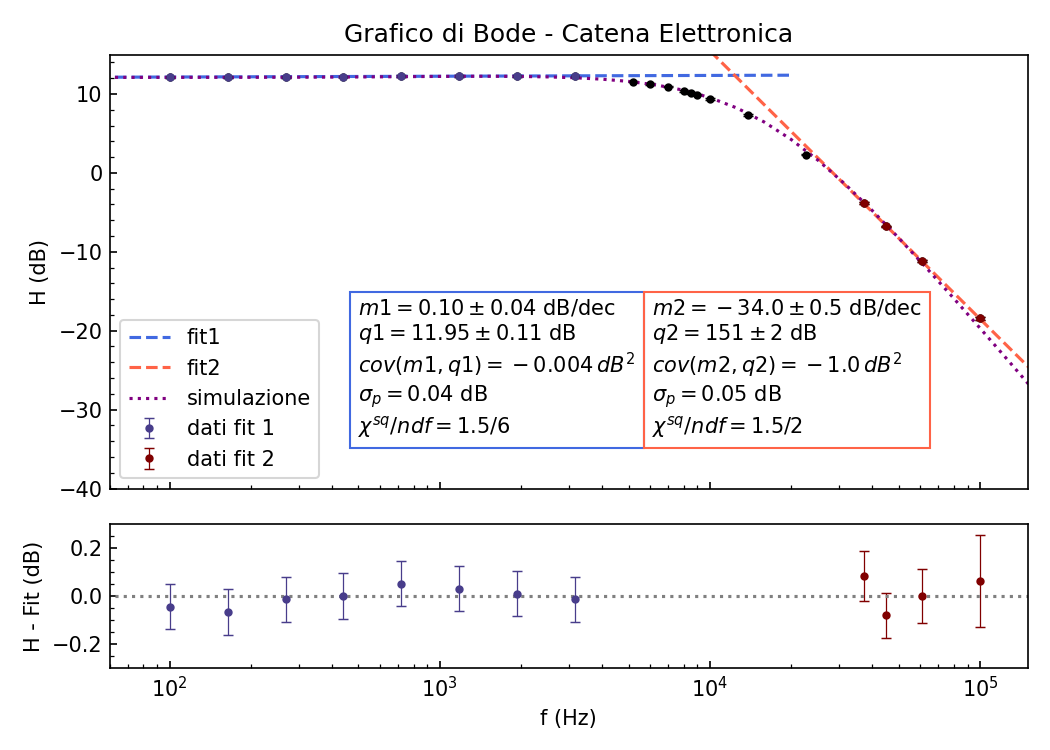
\includegraphics[width=0.8\textwidth]{../ampli/images/fit_bode}
\caption{\footnotesize{Grafico di Bode della catena elettronica completa e simulazione LTspice. Si mostrano anche i residui delle due interpolazioni da cui si è ricavata la frequenza di taglio.}}\label{fig:catena_fit_bode}
\end{figure}
%------------------------------------

\section{Conclusioni}
\label{sec:conclusioni}
La catena elettronica così prodotta permette quindi di trasformare il segnale
di corrente di un sensore di radiazione (che nel nostro caso è stato simulato da un'onda quadra in ingresso) in un segnale adatto ad un generico DAQ che lavora in un range attorno ai $2\V$. Tuttavia, analizzando singolarmente i moduli della catena, sono state osservate numerose discrepanze con le aspettative teoriche e con le simulazioni: in particolare, lo shaping time e la tensione massima prevista in output allo shaper risultano particolarmente anaomale. Conseguentemente, anche la frequenza di taglio della catena elettronica è incompatibile con quella prevista.   Questo rende il circuito realizzato non ottimale, soprattutto se confrontato a sistemi elettronici più complessi e costosi che sono in grado di gestire segnali anche piu piccoli e veloci grazie ad una banda più larga e ad una migliore gestione del rumore.


\end{document}
